\documentclass[11pt]{article}
\usepackage[T1]{fontenc}
\usepackage[utf8]{inputenc}
\usepackage[a4paper,margin=1in]{geometry}
\usepackage{lmodern}
\usepackage{amsmath,amssymb,mathtools}
\usepackage{booktabs,longtable,array}
\usepackage{enumitem}
\usepackage{xcolor}
\usepackage{hyperref}
\usepackage{tikz}
\usetikzlibrary{arrows.meta,positioning,shapes.geometric,fit}
\hypersetup{colorlinks=true,linkcolor=blue!50!black,urlcolor=blue!50!black}

\title{Virtual Staining and Early Fluorescence Prediction\\for Yichao Brightfield Organoid Imaging}
\author{OrganoidAgent}
\date{2026-06-27}

\newcommand{\B}{\mathbf{B}}
\newcommand{\F}{\mathbf{F}}
\newcommand{\M}{\mathbf{M}}
\newcommand{\Y}{\mathbf{Y}}
\newcommand{\R}{\mathbb{R}}
\newcommand{\E}{\mathbb{E}}
\newcommand{\argmin}{\operatorname*{arg\,min}}
\newcommand{\Dice}{\operatorname{Dice}}
\newcommand{\AUROC}{\operatorname{AUROC}}
\newcommand{\AUPRC}{\operatorname{AUPRC}}

\begin{document}
\maketitle
\tableofcontents

\section{Purpose}
The project goal should be framed more broadly than pixel-to-pixel fluorescence synthesis. The practical biological goal is to use label-free brightfield morphology to infer differentiation state, marker expression, or future marker expression in intestinal organoids. This report consolidates the current strategy into three staged tasks:
\[
\B_d \rightarrow \F_d,\qquad
\B_d \rightarrow \Y_d,\qquad
\B_k \rightarrow \Y_d \quad (k<d),
\]
where \(\B_d\) is brightfield at day \(d\), \(\F_d\) is fluorescence at day \(d\), and \(\Y_d\) can be a cleaned fluorescence image, a positive-expression mask, a cell-type map, or an organoid-level expression/composition score.

\section{Conversation-Derived Strategy}
The visible WeChat discussion suggests a pragmatic research sequence. If direct future fluorescence prediction is not reliable enough, the project can still be valuable as virtual staining or brightfield-based cell-type inference. The important biological observation is that the currently labeled fluorescent phenotype is likely a relatively distinguishable Goblet/high-goblet-like cell state. This should be the first target because it is easier than rare cell types and can establish whether label-free brightfield morphology contains useful information.

The discussion also identifies rarer cell types, such as Paneth cells and enteroendocrine cells, as biologically meaningful but data-limited. These should not be the first target unless targeted marker imaging or external pretraining data is available. A robust staged plan is therefore:
\begin{enumerate}[leftmargin=1.5em]
  \item prove same-day virtual staining on the currently labeled Goblet-like marker;
  \item convert the same-day task into a cell-type or expression-region inference task;
  \item only then test early-to-later prediction without future leakage;
  \item defer rare cell-type prediction until enough marker-specific data exists.
\end{enumerate}

\section{Scientific Context}
\subsection{In-silico labeling}
In-silico labeling directly supports this direction. Christiansen et al. showed that machine learning can infer fluorescent labels from unlabeled transmitted-light microscopy images across multiple biological settings \cite{christiansen2018}. Ounkomol et al. extended this idea to label-free prediction of three-dimensional fluorescence from transmitted-light microscopy \cite{ounkomol2018}. These papers justify the same-day Yichao task:
\[
\hat{\F}_{d}=f_{\theta}(\B_d).
\]
The key lesson is that not every label is equally predictable. The right first question is not whether all fluorescence can be perfectly reconstructed, but which marker or cell state is predictable above chance and useful enough for biological screening.

\subsection{Virtual staining}
Virtual histological staining is a related but broader field. Rivenson et al. demonstrated deep-learning virtual staining of label-free tissue autofluorescence images into histology-like outputs \cite{rivenson2019}. The imaging modality differs from Yichao's brightfield data, but the logic is the same: a trained network can produce staining-like biological readouts from minimally invasive imaging.

\subsection{Label-free organoid analysis}
Organoid-specific label-free analysis is also emerging. LabelFreeTracker uses U-Net-style models trained on brightfield and fluorescence images of 3D mouse intestinal organoids to infer nuclei and membranes \cite{labelFreeTracker2025}. Reviews of label-free live-cell recognition emphasize that brightfield and related label-free modalities can support segmentation, tracking, and biological readouts without perturbing the sample \cite{chen2024}. This makes the Yichao task technically plausible, especially for morphology-rich Goblet-like phenotypes.

\subsection{Cell-type biology}
The Gut Cell Atlas and associated single-cell atlas work describe intestinal epithelial cell types across space and time, including BEST4 cells, enterocytes/colonocytes, enteroendocrine cells, Goblet cells, Paneth cells, Tuft cells, transit-amplifying cells, and stem cells \cite{gutcellatlas,elmentaite2021}. These references should guide which marker labels are requested in future experiments. They do not by themselves provide paired brightfield-to-fluorescence supervision, but they define the biological target space.

\section{Three-Level Prediction Model}
\subsection{Level 1: Same-day fluorescence prediction}
The first trainable task is same-day B2F:
\[
\hat{\F}_{i,d}=f_{\theta}(\B_{i,d}),
\]
where \(i\) indexes a segmented organoid instance. This task validates channel mapping, segmentation, registration, target cleaning, and morphology-to-marker signal.

\subsection{Level 2: Same-day virtual staining / cell-type inference}
The second task is segmentation-like inference:
\[
(\hat{\M}_{i,d}, \hat{S}_{i,d}) = g_{\theta}(\B_{i,d}),
\]
where \(\M\) is a positive-expression mask and \(S\) is an organoid-level expression score or cell-type composition vector. This is often more useful than pixel-perfect fluorescence regression because fluorescence intensity can be confounded by overexposure, background, debris, or acquisition differences.

\subsection{Level 3: Early-to-later prediction}
The final target is:
\[
(\hat{\M}_{i,d|k}, \hat{S}_{i,d|k}, \hat{\F}_{i,d|k})
= h_{\theta}(\B_{i,k}, \Delta),\qquad \Delta=d-k,\quad k<d.
\]
The horizon \(\Delta\) is allowed as input because the requested forecast time is known. Future fluorescence, future brightfield, and future-derived normalization statistics are not allowed as input.

\section{Data Preparation}
For the new Yichao v2 data, training should not begin until channel mapping is visually confirmed. The current v2 inventory is:

\begin{longtable}{@{}p{0.30\linewidth}p{0.16\linewidth}p{0.16\linewidth}p{0.26\linewidth}@{}}
\caption{Yichao v2 preparation status.}\label{tab:v2}\\
\toprule
Folder & Day hint & Current state & Main risk\\
\midrule
\endfirsthead
\toprule
Folder & Day hint & Current state & Main risk\\
\midrule
\endhead
1\_N39Rep\_Globet\_DF\_D3 & D3 & extracted/grouped & confirm channel map\\
2\_N39Rep\_Globet\_DF\_D4 & D4 & extracted/grouped & confirm channel map\\
3\_N39Rep\_Globet\_DF\_D2 & D2 & copied/metadata & generic series, 7 channels\\
4\_N39Rep\_Globet\_DF\_D3\_1 & D3 & copied/metadata & generic series, 8 channels\\
5\_N39Rep\_Globet\_DF\_D3\_2 & D3 & copied/metadata & generic series, 8 channels\\
\bottomrule
\end{longtable}

The preparation pipeline should be:
\begin{enumerate}[leftmargin=1.5em]
  \item extract all LIF planes;
  \item build channel contact sheets;
  \item manually confirm brightfield and Alexa488/green fluorescence channels;
  \item project or choose z according to a documented rule;
  \item segment the brightfield image, not the fluorescence image;
  \item crop paired brightfield, cleaned fluorescence, and mask targets;
  \item store every crop in a database with day, field, channel map, z policy, object id, edge-padding flag, crop size, and split group.
\end{enumerate}

\section{Recommended Target Construction}
The fluorescence target should be split into a continuous cleaned signal and a positive mask:
\[
\F^{clean} = \operatorname{clean}(\F),\qquad
\M^{clean} = \mathbf{1}\{\F^{clean}>\tau\}.
\]
The mask handles localization and severe positive/negative imbalance. The continuous target preserves intensity realism and prevents the model from learning only binary blobs.

A practical same-day objective is:
\[
\mathcal{L}_{same}
=
\lambda_M\mathcal{L}_{mask}(\hat{\M}, \M^{clean})
+\lambda_F\left\|\M^{clean}\odot(\hat{\F}-\F^{clean})\right\|_1
+\lambda_S\left|\hat{S}-S\right|.
\]
\(\mathcal{L}_{mask}\) should include Dice or focal/BCE terms because positive pixels are sparse \cite{lin2017}. \(S\) can be total positive fluorescence, mean positive fluorescence, positive fraction, or a Goblet-like expression score.

\section{Temporal Objective Without Future Leakage}
For early prediction, define:
\[
\mathcal{D}_{future}=\{(i,k,d): k<d,\; i \text{ belongs to a valid split group}\}.
\]
The model predicts later targets from earlier brightfield:
\[
\hat{\Y}_{i,d|k}=h_{\theta}(\B_{i,k}, d-k).
\]
The loss is:
\[
\mathcal{L}_{future}
=
\sum_{(i,k,d)\in\mathcal{D}_{future}}
w(d-k)\,
\mathcal{L}_{target}(\hat{\Y}_{i,d|k},\Y_{i,d}).
\]
The early horizon should be encouraged but not over-forced. A simple fixed weight is:
\[
w(\Delta)=\exp(-\gamma \Delta).
\]
A stronger option is learned uncertainty weighting:
\[
\mathcal{L}_{\Delta}
=
\frac{\mathcal{L}_{raw,\Delta}}{2\sigma_\Delta^2}
+\log\sigma_\Delta.
\]
This lets the model assign higher uncertainty to horizons where morphology genuinely cannot determine future expression.

\section{No-Leakage Rules}
Temporal prediction requires stricter splitting than same-day image translation:
\begin{enumerate}[leftmargin=1.5em]
  \item split by biological field, position, replicate, or lineage before making temporal pairs;
  \item keep all days and acquisitions from the same split group in one split;
  \item for \(B_k \rightarrow Y_d\), use only information available at or before \(k\);
  \item fit normalization, thresholds, and target cleaning only on training data;
  \item choose the earliest useful day on validation data only;
  \item reserve at least one acquisition batch as an external test when possible.
\end{enumerate}

\section{Evaluation}
The output should not be judged only by whole-image loss. Use a tiered evaluation:

\begin{longtable}{@{}p{0.24\linewidth}p{0.32\linewidth}p{0.34\linewidth}@{}}
\caption{Recommended evaluation metrics.}\label{tab:metrics}\\
\toprule
Level & Metric & Meaning\\
\midrule
\endfirsthead
\toprule
Level & Metric & Meaning\\
\midrule
\endhead
Pixel/region & Dice, IoU, precision, recall & whether positive expression regions are localized\\
Continuous signal & masked MAE, Pearson/Spearman & whether predicted intensity follows real fluorescence\\
Organoid level & total expression correlation, calibration & whether expression score is useful for screening\\
Classification & \(\AUROC\), \(\AUPRC\), balanced accuracy & whether fluorescent/Goblet-like organoids are distinguished\\
Temporal & earliest useful day \(k^*\) & how early prediction becomes reliable\\
\bottomrule
\end{longtable}

The earliest useful day is:
\[
k^*=\min k \quad \text{s.t. validation metrics exceed predefined thresholds across split groups.}
\]

\section{Recommended Roadmap}
\begin{center}
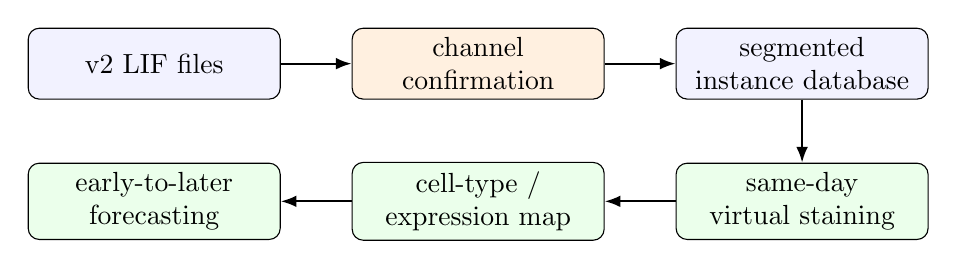
\begin{tikzpicture}[
  node distance=0.8cm and 0.9cm,
  box/.style={draw, rounded corners, align=center, minimum width=3.2cm, minimum height=0.9cm, fill=blue!5},
  warn/.style={draw, rounded corners, align=center, minimum width=3.2cm, minimum height=0.9cm, fill=orange!12},
  model/.style={draw, rounded corners, align=center, minimum width=3.2cm, minimum height=0.9cm, fill=green!8},
  arrow/.style={-{Latex[length=2mm]}, thick}
]
\node[box] (v2) {v2 LIF files};
\node[warn, right=of v2] (map) {channel\\confirmation};
\node[box, right=of map] (db) {segmented\\instance database};
\node[model, below=of db] (same) {same-day\\virtual staining};
\node[model, left=of same] (class) {cell-type /\\expression map};
\node[model, left=of class] (future) {early-to-later\\forecasting};
\draw[arrow] (v2) -- (map);
\draw[arrow] (map) -- (db);
\draw[arrow] (db) -- (same);
\draw[arrow] (same) -- (class);
\draw[arrow] (class) -- (future);
\end{tikzpicture}
\end{center}

The immediate next experiment should be conservative: confirm v2 channels, build a v2 instance database, and train a same-day Goblet-like virtual-staining model. Only if same-day prediction is clearly above chance should the temporal \(D2\rightarrow D3/D4\) or \(D3\rightarrow D4\) task be trained.

\section{Conclusion}
The most robust interpretation of the current project is not ``pix2pix fluorescence generation'' alone. It is label-free virtual staining for a biologically meaningful epithelial differentiation marker, followed by no-leakage early prediction. The first target should be the current Goblet/high-expression phenotype because it is visible, biologically relevant, and experimentally available. Rare cell types should be handled later with targeted labels or external data.

\begin{thebibliography}{9}

\bibitem{christiansen2018}
Christiansen, E. M. et al.
\newblock In Silico Labeling: Predicting Fluorescent Labels in Unlabeled Images.
\newblock \emph{Cell}, 173, 792--803.e19, 2018.
\newblock \url{https://pubmed.ncbi.nlm.nih.gov/29656897/}

\bibitem{ounkomol2018}
Ounkomol, C. et al.
\newblock Label-free prediction of three-dimensional fluorescence images from transmitted-light microscopy.
\newblock \emph{Nature Methods}, 15, 917--920, 2018.
\newblock \url{https://www.nature.com/articles/s41592-018-0111-2}

\bibitem{rivenson2019}
Rivenson, Y. et al.
\newblock Virtual histological staining of unlabelled tissue-autofluorescence images via deep learning.
\newblock \emph{Nature Biomedical Engineering}, 3, 466--477, 2019.
\newblock \url{https://www.nature.com/articles/s41551-019-0362-y}

\bibitem{labelFreeTracker2025}
Kok, R. N. U. et al.
\newblock Label-free cell imaging and tracking in 3D organoids.
\newblock \emph{Cell Reports Physical Science}, 2025.
\newblock \url{https://www.cell.com/cell-reports-physical-science/pdfExtended/S2666-3864%2825%2900121-3}

\bibitem{chen2024}
Chen, B. et al.
\newblock Label-free live cell recognition and tracking for biological discoveries and translational applications.
\newblock \emph{npj Imaging}, 2, 41, 2024.
\newblock \url{https://www.nature.com/articles/s44303-024-00046-y}

\bibitem{gutcellatlas}
Gut Cell Atlas.
\newblock \url{https://www.gutcellatlas.org/}

\bibitem{elmentaite2021}
Elmentaite, R. et al.
\newblock Cells of the human intestinal tract mapped across space and time.
\newblock \emph{Nature}, 597, 250--255, 2021.
\newblock \url{https://www.nature.com/articles/s41586-021-03852-1}

\bibitem{ronneberger2015}
Ronneberger, O., Fischer, P. and Brox, T.
\newblock U-Net: Convolutional Networks for Biomedical Image Segmentation.
\newblock MICCAI, 2015.
\newblock \url{https://arxiv.org/abs/1505.04597}

\bibitem{lin2017}
Lin, T.-Y. et al.
\newblock Focal Loss for Dense Object Detection.
\newblock ICCV, 2017.
\newblock \url{https://arxiv.org/abs/1708.02002}

\end{thebibliography}

\end{document}
